\newpage

\appendix

\section{Large Language Model Usage}
In this paper, Large Language Models (LLMs) are used exclusively for grammatical error correction.

%%%%%%%%%%%%%%%%%%%%%%%%%%%%%%%%%%%%%%%%%%%%%%%%%%%%%%%%%
\section{Layer Selection and Generalizability}
\label{appendix_generalizability}

% 
\begin{figure*}[h]
  \centering
  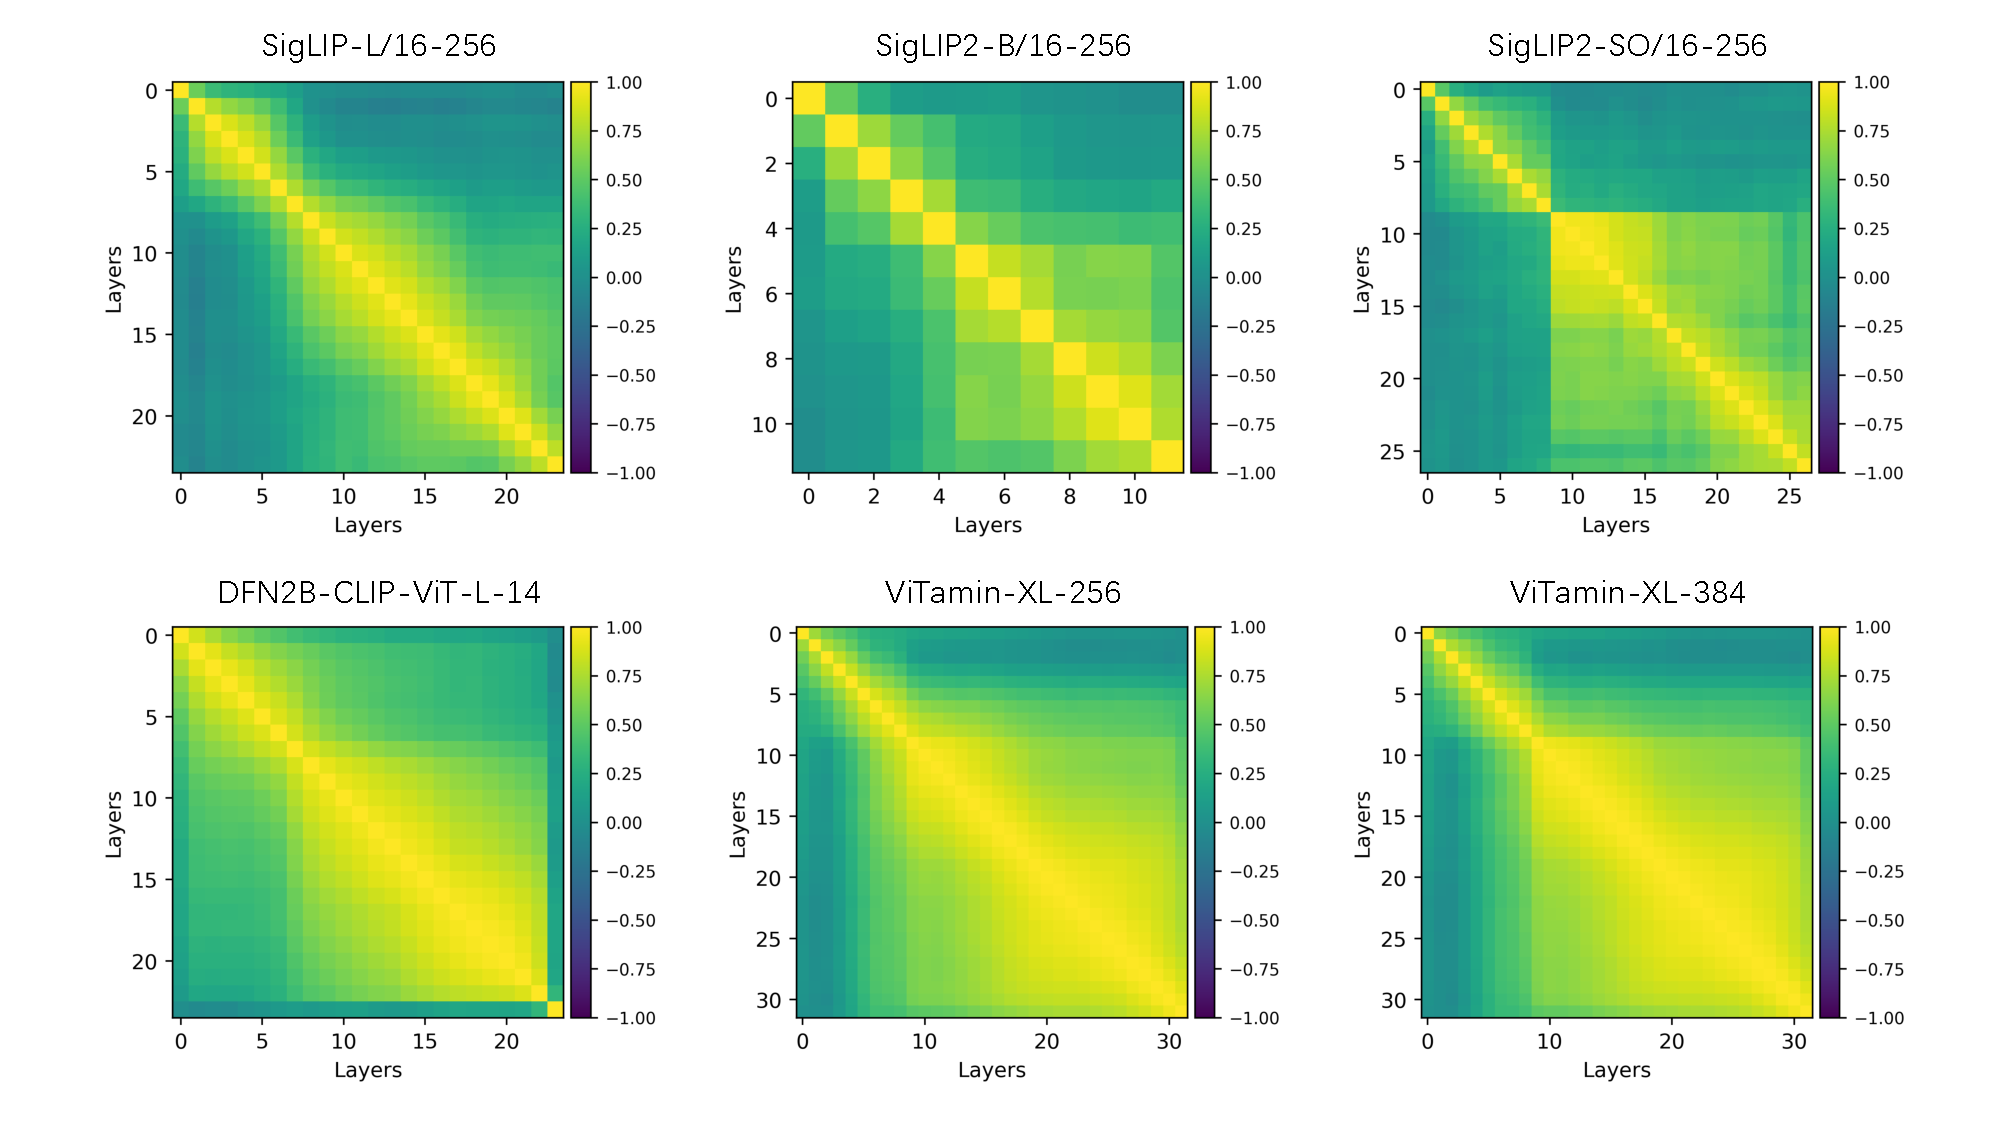
\includegraphics[width=0.8\textwidth]{iclr2026/imgs/visualization.pdf}
  \caption{
      Additional visualizations of inter-layer cosine similarity across different backbones, revealing a consistent hierarchical pattern across architectures, model scales, and resolutions. A cohesive high-similarity region corresponding to the shallow layers can be clearly observed.
  }
  \label{fig:visualization_appendix}
\end{figure*}


As discussed in Sec.~\ref{sec:method_tokenizer}, we can partition the vision encoder into shallow and deep regions based on the cosine similarity between layers (see Fig.~\ref{tab:cluster} and Appendix~\ref{partitioning}). Empirically, selecting the last layer within the shallow region, typically corresponding to \textit{the first quarter to third of layers}, yields the best results.
As validated in the main text, our method successfully generalizes across multiple backbones, including SigLIP-L/16-256, SigLIP-SO/14-384, and SigLIP2-SO/16-256. 


\begin{figure*}[h]
  \centering
  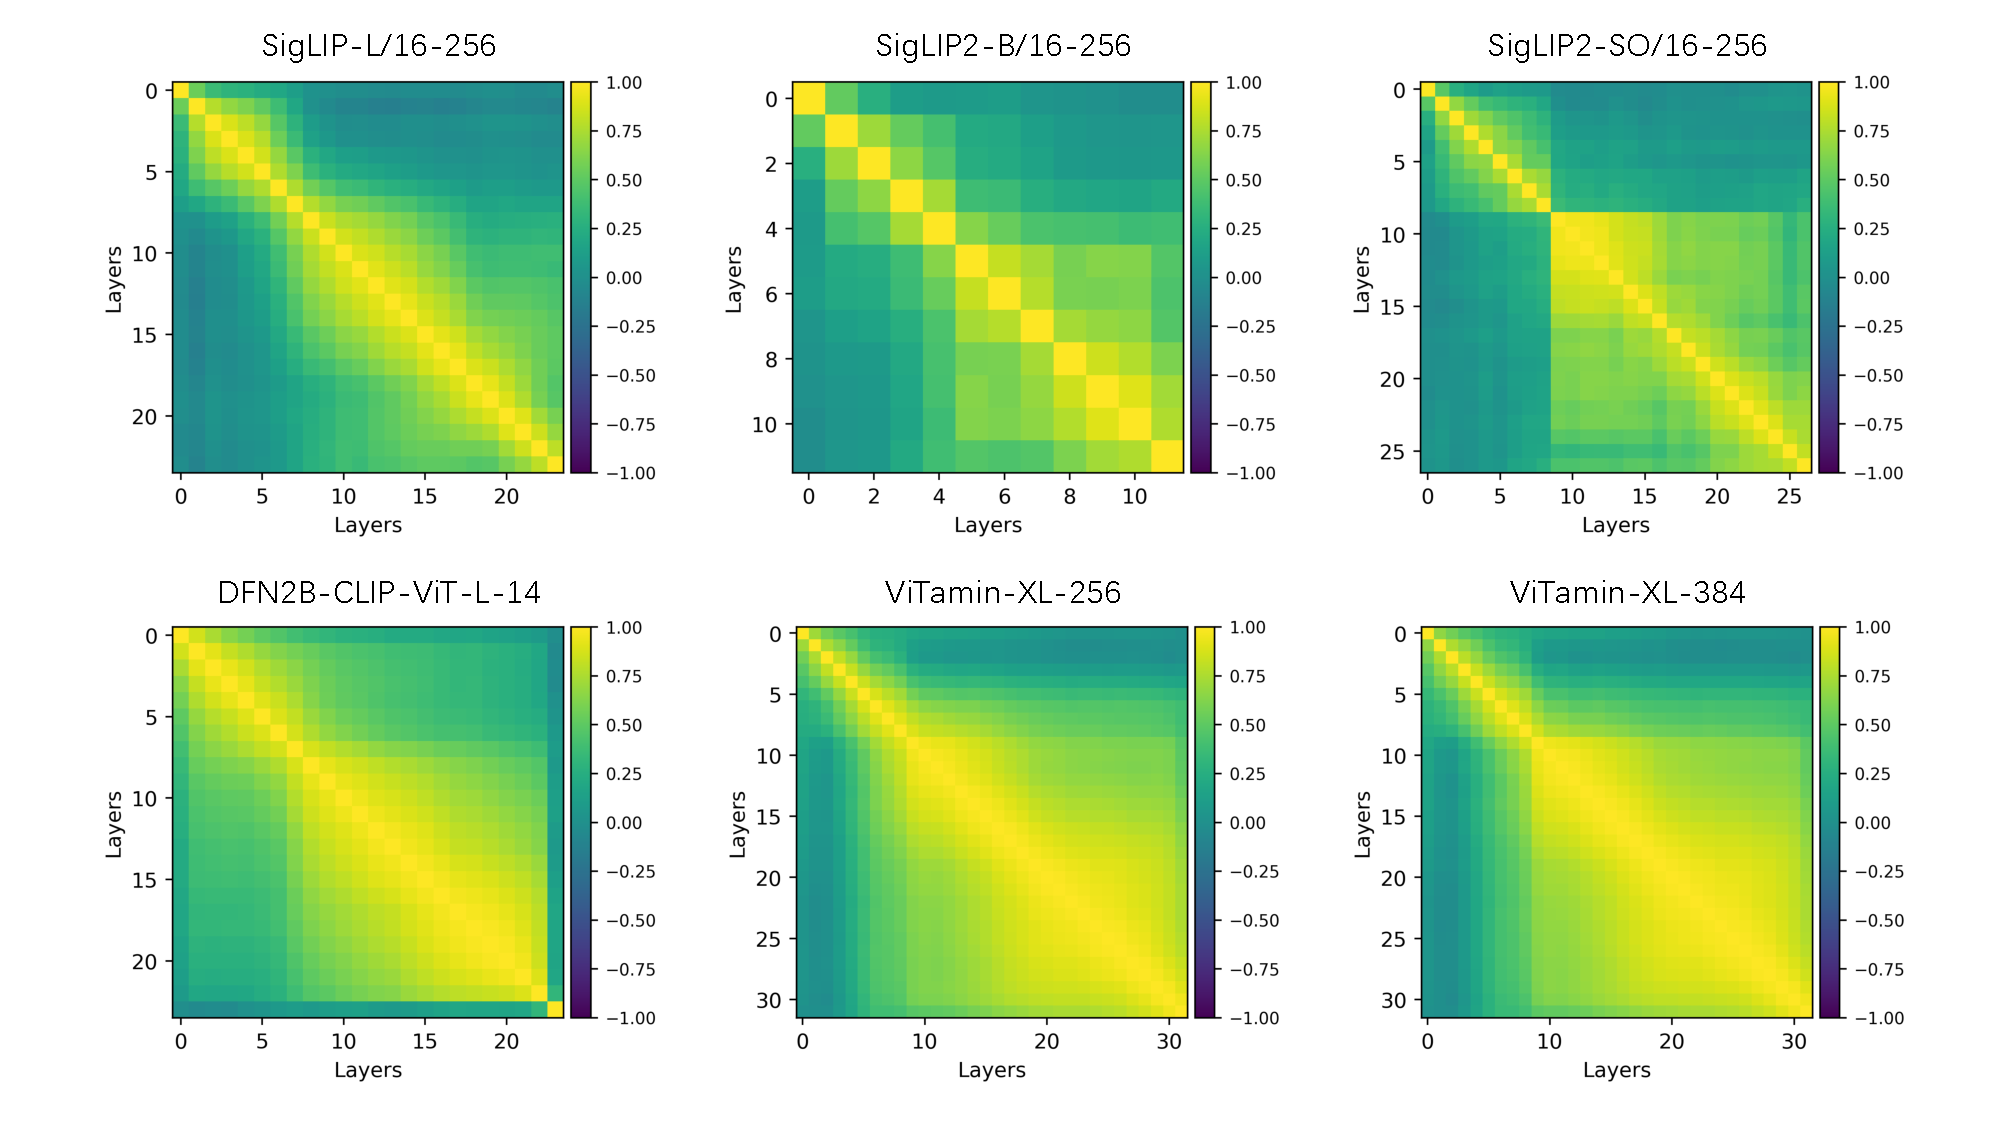
\includegraphics[width=0.8\textwidth]{iclr2026/imgs/visualization.pdf}
  \caption{
      Additional visualizations of inter-layer cosine similarity across different backbones, revealing a consistent hierarchical pattern across architectures, model scales, and resolutions. A cohesive high-similarity region corresponding to the shallow layers can be clearly observed.
  }
  \label{fig:visualization_appendix}
\end{figure*}


To further strengthen our claim, we include a comprehensive validation of the method’s generalizability, covering six mainstream backbones—OpenAI’s CLIP~\citep{radford2021clip}, Apple’s DFN~\citep{fang2023dfn}, BAAI’s EVA~\citep{eva02}, Google’s SigLIP~\citep{zhai2023siglip}, SigLIP2~\citep{tschannen2025siglip2}, and the hybrid CNN–Transformer architecture ViTamin~\citep{chen2024vitamin}—under consistent settings (RVQ = 8, codebook size = 16,384, 2M training samples). Our findings are summarized as follows.

\textbf{(1) Ablations on model backbones and model size.}~~As shown in Table.\ref{tab:backbones} and Table.\ref{tab:model_size}, across all tested backbones with varying types and total layer counts, selecting the \textit{first quarter of layers} for reconstruction consistently yields the best reconstruction quality and semantic performance.

\begin{minipage}[h]{0.29\textwidth}
    \centering
    \captionsetup{type=table}
    \caption{Model backbone.}
    \label{tab:backbones}
    % \tablestyle{3pt}{1.15}
    \tablestyle{2pt}{1.175}
    \resizebox{\linewidth}{!}{
    \begin{tabular}{lcccccc}
        \toprule
        Backbone & Layer recon./total & Zero-shot & rFID \\
        \hline
        & 6/24 & \textbf{79.2} & \textbf{0.84} \\
        DFN-L/14-224 & 12/24 & 77.1 & 1.35 \\
        & 18/24 & 72.2 & 3.25 \\
        \hline
        & 6/24 & \textbf{77.8} & \textbf{0.80} \\
        EVA-02-L/14-224& 12/24 & 75.2 & 1.16 \\
        & 18/24 & 69.9 & 3.22 \\
        \hline
        & 6/24 & \textbf{73.2} & \textbf{0.87} \\
        CLIP-L/14-224& 12/24 & 70.8 & 1.80 \\
        & 18/24 & 65.5 & 3.58 \\
        \hline
        & 6/24 & \textbf{78.8} & \textbf{0.78} \\
        SigLIP-L/16-256& 12/24 & 76.3 & 1.27 \\
        & 18/24 & 72.9 & 2.61 \\
        \hline
        & 6/24 & \textbf{80.4} & \textbf{0.72} \\
        SigLIP2-L/16-256& 12/24 & 77.6 & 1.09 \\
        & 18/24 & 72.9 & 2.93 \\
        \hline
        & 6/24 & \textbf{80.0} & \textbf{0.39} \\
        ViTamin-XL-384& 12/24 & 78.6 & 0.88 \\
        & 18/24 & 73.8 & 2.25 \\
        \bottomrule
    \end{tabular}}
\end{minipage}
\hfill
\begin{minipage}[h]{0.355\textwidth}
    \centering
    \captionsetup{type=table}
    \caption{Model size and total layer.}
    \label{tab:model_size}
    % \tablestyle{3pt}{1.15}
    \tablestyle{2pt}{1.175}
    \resizebox{\linewidth}{!}{
    \begin{tabular}{lcccccc}
        \toprule
        Backbone & Layer recon./total & Zero-shot & rFID \\
        \hline
        & 3/12 & \textbf{74.1} & \textbf{0.98} \\
        DFN-B/16-224  & 6/12 & 71.4 & 1.58 \\
        & 9/12 & 66.1 & 3.21 \\
        \hline
        & 6/24 & \textbf{79.2} & \textbf{0.84} \\
        DFN-L/14-224 & 12/24 & 77.1 & 1.35 \\
        & 18/24 & 72.2 & 3.25 \\
        \hline
        & 8/32 & \textbf{81.0} & \textbf{0.73} \\
        DFN-H/14-224 & 16/32 & 79.5 & 1.28 \\
        & 24/32 & 74.3 & 2.78 \\
        \hline
        & 6/24 & \textbf{80.4} & \textbf{0.72} \\
        SigLIP2-L/16-256 & 12/24 & 77.6 & 1.09 \\
        & 18/24 & 72.9 & 2.93 \\
        \hline
        & 7/27 & \textbf{81.2} & \textbf{0.69} \\
        SigLIP2-SO/16-256 & 14/27 & 78.4 & 1.08 \\
        & 21/27 & 73.7 & 3.02 \\
        \bottomrule
    \end{tabular}}
\end{minipage}
\hfill
\begin{minipage}[h]{0.335\textwidth}
    \centering
    \captionsetup{type=table}
    \caption{Robustness on layers.}
    \label{tab:robustness}
    % \tablestyle{3pt}{1.15}
    \tablestyle{2pt}{1.175}
    \resizebox{\linewidth}{!}{
    \begin{tabular}{lcccccc}
        \toprule
        Backbone & Layer recon./total & Zero-shot & rFID \\
        \hline
        \multirow{2}{*}{DFN-B/16-224} & 3/12 & \textbf{74.1} & 0.98 \\
        & 4/12 & 73.9 & \textbf{0.97} \\
        \hline
        \multirow{3}{*}{DFN-L/14-224} & 5/24 & 79.0 & \textbf{0.82} \\
        & 6/24 & \textbf{79.2} & 0.84 \\
        & 7/24 & 78.9 & 0.84 \\
        \hline
        \multirow{3}{*}{DFN-H/14-224} & 6/32 & \textbf{81.1} & 0.73 \\
        & 8/32 & 81.0 & 0.73 \\
        & 10/32 & 80.7 & \textbf{0.72} \\
        \hline
        \multirow{3}{*}{SigLIP2-L/16-256} & 5/24 & 80.4 & 0.74 \\
        & 6/24 & \textbf{80.4} & \textbf{0.72} \\
        & 7/24 & 80.2 & 0.75 \\
        \hline
        \multirow{5}{*}{SigLIP2-SO/16-256} & 5/27 & 81.0 & 0.70 \\
        & 6/27 & 81.2 & \textbf{0.66} \\
        & 7/27 & 81.2 & 0.69 \\
        & 8/27 & \textbf{81.3} & 0.67 \\
        & 9/27 & 81.0 & 0.72 \\
        \bottomrule
    \end{tabular}}
\end{minipage}

\textbf{(2) Robustness to specific layer choice.}~~As shown in Table.~\ref{tab:robustness}, our method remains stable as long as the reconstruction layers lie roughly within the first quarter of the network. Minor shifts (\(\pm1\)–\(2\) layers) cause negligible changes, confirming its robustness and broad applicability.

These findings indicate that for a new ViT architecture, one can confidently select the first quarter of layers for reconstruction to achieve optimal results.
Moreover, As shown in Fig.~\ref{fig:visualization_appendix}, we also provide more visualizations of inter-layer cosine similarity across backbones, revealing a consistent hierarchical pattern divisible into shallow and deep layers (also supported by prior study~\citep{chen2025rethinking}), further supporting the universality of our method.

%%%%%%%%%%%%%%%%%%%%%%%%%%%%%%%%%%%%%%%%%%%%%%%%%%%%%%%%%
\section{Discussion and Comparison with UniTok}
\label{appendix_unitok}

Since UniTok adopts a more advanced visual backbone, decoder, and discriminator architecture, we conduct a fair comparison by re-training our DualToken under the same encoder and decoder settings used in UniTok, \textit{i.e.}, choosing ViTamin-L/16, a hybrid architecture of CNN and transformer, to instantiate DualToken.
Under this setup, DualToken achieves stronger semantic performance and competitive reconstruction quality, as evidenced by the comparison between (a) and (b) in Table~\ref{tab:unitok}.


\begin{table}[ht]
\centering
\caption{Comparison with UniTok.}
\label{tab:unitok}
\begin{tabular}{lcc}
\toprule
Tokenizer & rFID $\downarrow$ & Zero-Shot Acc $\uparrow$ \\
\midrule
(a) UniTok              & 0.38 & 78.6 \\
(b) DualToken (RVQ)     & 0.39 & 80.3 \\
(c) DualToken (MCQ)     & 0.25 & 82.2 \\
\bottomrule
\end{tabular}
\end{table}

Furthermore, \emph{DualToken and UniTok are complementary}. Specifically, by replacing our original RVQ quantizer with UniTok’s proposed \textbf{MCQ}, we observe consistent improvements in both reconstruction fidelity and zero-shot classification, as evidenced by the comparison between (b) and (c) in Table~\ref{tab:unitok}.

These results suggest that future work may benefit from \textbf{integrating our dual visual vocabulary} formulation with more advanced quantizers such as MCQ.

% %%%%%%%%%%%%%%%%%%%%%%%%%%%%%%%%%%%%%%%%%%%%%%%%%%%%%%%%%
% \section{Great Potential in Native Multimodal Interleaved CoT}
% \label{appendix_interleave}

%%%%%%%%%%%%%%%%%%%%%%%%%%%%%%%%%%%%%%%%%%%%%%%%%%%%%%%%%
\section{Computational Analysis}
\label{appendix_computation}

Introducing two codebooks \textbf{DOES NOT} significantly increase the computational overhead, demonstrated by two aspects: \textbf{parameter count} and \textbf{memory usage with inference latency}.

\subsection{Parameter Count}

The ONLY additional parameters arise from 3 components:
\begin{itemize}[leftmargin=*]
    \item The MLP projector's dimension changes from (1024$\rightarrow$2048$\rightarrow$2048) to (2048$\rightarrow$2048$\rightarrow$2048), which adds \textbf{2.1M} parameters.
    \item An additional visual head: \textbf{258M} parameters.
    \item An additional VQEmbedding layer: \textbf{16M} parameters.
\end{itemize}

Together, these account for only \textbf{8.93\%} of the total parameters compared to the LLM backbone (3B). When scaling to larger backbones (e.g., 7B), the relative impact becomes even more negligible.

\subsection{Memory Usage and Inference Latency}

Since our dual tokens are concatenated along feature dimension rather than sequence dimension, and the input dimension to the LLM remains unchanged, \textbf{no new pathway is introduced to the LLM}, and the computational cost of the LLM backbone remains strictly the same. The only increase stems from the components listed above.

\begin{table}[ht]
\centering
\caption{Memory Usage and Inference Latency}
\label{tab:memory}
\begin{tabular}{lccc}
\toprule
 & Training Memory Usage & Inference Time Cost & Single Forward GFLOPs \\
\midrule
single token & 73.8G & 11.42s & 328.98 \\
dual token   & 78.2G & 12.97s & 337.20 \\
\bottomrule
\end{tabular}
\end{table}

Memory usage is measured under the same local batch size and device. FLOPs and inference time are averaged on T2I task (256px) over the MJHQ-30K dataset. Statistics for the VQA task have also been added to the paper.


%%%%%%%%%%%%%%%%%%%%%%%%%%%%%%%%%%%%%%%%%%%%%%%%%%%%%%%%%
\section{Results on More Generation Benchmarks}
\label{appendix_genbench}

Following VILA-U, we report results on GenAI-Bench and MJHQ-30K in the main text. We now extend our evaluation to include GenEval~\citep{ghosh2023geneval} and WISE~\citep{niu2025wise}. The results demonstrate that DualToken achieves competitive performance across both benchmarks.

\begin{table}[ht]
\centering
\caption{Evaluation results on GenEval and WISE benchmarks.}
\label{tab:geneval-wise}
    \tablestyle{2pt}{1.1}
    \resizebox{0.7\linewidth}{!}{
    \begin{tabular}{lcc}
    \toprule
    Model & GenEval (Overall) $\uparrow$ & WISE (Overall) $\uparrow$ \\
    \midrule
    SDv1.5~\citep{latentdiffusion}           &0.43  &0.32 \\
    SDXL~\citep{sdxl}             &0.55  &0.43 \\
    Chameleon-7B~\citep{team2024chameleon}     &0.39  &-    \\
    EMU3-8B~\citep{wang2024emu3}          &0.66  &0.39 \\
    Janus~\citep{wu2024janus}            &0.61  &0.23 \\
    Janus-Pro-7B~\citep{chen2025januspro}     &0.80  &0.35 \\
    ILLUME-7B~\citep{wang2024illume}        &0.61  &-    \\
    TokenFlow-XL-14B~\citep{qu2024tokenflow} &0.63  &-    \\
    Muse-VL-7B~\citep{xie2025musevl}       &0.57  &-\\
    UniToken-7B~\citep{jiao2025unitoken}      &0.63  &-\\
    Show-o2-1.5B~\citep{xie2025showo2}     &0.73  &0.35\\
    Show-o2-7B~\citep{xie2025showo2}       &0.76  &0.39\\
    VILA-U-7B~\citep{wu2025vilau}        &-     &0.31 \\
    \compare{}DualToken-3B     &\compare{}0.72  &\compare{}0.35\\
    \compare{}DualToken-7B     &\compare{}0.75  &\compare{}0.39\\
    \bottomrule
    \end{tabular}}
\end{table}


%%%%%%%%%%%%%%%%%%%%%%%%%%%%%%%%%%%%%%%%%%%%%%%%%%%%%%%%%
\section{Implementation Details}
\label{appendix_implementation}

\subsection{Partitioning of the SigLIP Encoder}
\label{partitioning}

We feed the ImageNet-1K~\citep{deng2009imagenet} validation set into SigLIP-SO400M-Patch14-384~\citep{zhai2023siglip}. For each image, we extract the representations from all layers of the model, each with a shape of $729\times1152$. Then, we apply average pooling along the spatial dimension (the first axis) of each layer's representation, resulting in a 1152-dimensional vector per layer.

Specifically, for each image, we obtain feature vectors from 26 layers, and compute the pairwise cosine similarity between these layer-wise representations to construct a $26\times26$ cosine similarity matrix.
To capture the overall similarity structure across layers in the model, we average the cosine similarity matrices across all images. The final similarity matrix $S^*$ is computed as:
\begin{equation}
\begin{aligned}
    S^* = \frac{1}{n} \sum_{i=1}^{n} S_i
\end{aligned}
\end{equation}

where $S_i$ denotes the cosine similarity matrix for the $i-th$ image, and $n$ is the total number of images. $S^*$ thus represents the average inter-layer similarity across the dataset.

\subsection{Image Clustering}
We extract intermediate representations from the 6th and 26th layers of SigLIP-SO400M-Patch14-384~\citep{zhai2023siglip} for each image in the ImageNet-1K validation set~\citep{deng2009imagenet}. The original representation shape is $729 \times 1152$, and we apply average pooling along the spatial dimension to obtain a single 1152-dimensional feature vector per image.
For both the 6th-layer and 26th-layer features, we perform k-means clustering with 1000 cluster centers (Cluster 0 to Cluster 999). The cluster analysis reveals that shallow-layer features (from the 6th layer) tend to capture low-level visual attributes such as texture and color, while deep-layer features (from the 26th layer) predominantly encode high-level semantic content.
The implementation code is provided in the \textit{supplementary material}, and additional visualizations are presented in Fig.~\ref{fig:cluster_appendix}.


\begin{figure*}[ht]
  \centering
  \includegraphics[width=\textwidth]{imgs/clustering.pdf}
  \caption{
      More visualizations of image clusters derived from features of (a) the 6th layer and (b) the 26th layer of SigLIP. Features from deep layers primarily cluster images based on high-level semantic content, whereas shallow-layer features tend to group images according to appearance-level cues such as color and texture.
      For instance, Cluster 17 contains images with similar scaly textures, while Clusters 60 and 110 predominantly group images by dominant colors (e.g., red or blue).
  }
  \label{fig:cluster_appendix}
\end{figure*}


\subsection{UMAP Feature Space Visualization}

We perform dimensionality reduction using UMAP to visualize the feature spaces from DualToken's 6th and 26th layers, as well as those from MoVQGAN and SigLIP. Specifically, we sample 1,000 images from the ImageNet-1K validation set and visualize the UMAP projections of their encoded features from each model. To ensure a fair comparison among the different visual models, all extracted features are first flattened and then uniformly processed via adaptive average pooling to maintain consistent dimensionality.

\subsection{Model Implementation Details}
\label{implement}

Our backbone model is built upon a decoder-only transformer architecture, and adopt Qwen2.5~\citep{yang2024qwen2d5} as our initialization due to its strong performance and public availability. The model uses RMSNorm\cite{zhang2019rms} for normalization.
For visual inputs to the LLM, we apply a projector to map the visual tokens into the same embedding space as the LLM. When predicting image tokens, the output hidden states of the LLM are passed through two separate projectors to align with the dimension of the semantic visual head and the pixel visual head. Each projector consists of two linear layers with a GeLU activation in between. We use special tokens---<image\_gen\_start> and <image\_gen\_end>---to indicate the boundaries of the image to be generated.

For visual heads, since residual quantization introduces a depth-stacked structure of codes at each visual position $p$, we implement our visual heads based on the depth transformer from RQ-VAE~\citep{lee2022rqvae}. 
Unlike the original depth transformer, which employs a single head to predict logits across all depths, we introduce separate classification heads to compute the logits for residuals at each corresponding depth~\citep{li2025baichuanaudio}.
As shown in Fig.\ref{fig:frameworks}, the semantic tokens and pixel tokens are processed by independent visual heads---the pixel head and the semantic head. Both heads share the same structure, comprising three layers of depth transformers and corresponding classification head for each depth.
Detailed training hyper-parameters are provided in Table~\ref{tab:hyper_params}.

\belowrulesep=0pt\aboverulesep=0pt

\begin{table}[t]
\centering
\tablestyle{2.5pt}{1.2}
\caption{Training hyper-parameters.}
\resizebox{1\textwidth}{!}{
    \begin{tabular}{l|c|ccccc}
    \toprule
    &\multirow{2}{*}{\shortstack{Visual\\Tokenizer}} & \multicolumn{5}{c}{MLLM} \\
    \cmidrule{3-7}
     \multirow{-2}[0]{*}{Settings} &                          &Stage 1                         &Stage 2         &Stage 3               &Stage 4-1      &Stage 4-2\\ 
    \midrule
    \multirow{2}{*}{Learning Rate}  &\multirow{2}{*}{7.2e-5}   &\multirow{2}{*}{Projector 1e-3} &Projector 2e-5  &Projector (Gen) 1e-4  &\multicolumn{2}{c}{All Projectors 1e-5}\\
    &                                                         &                                &LLM 2e-5        &Visual Heads 1e-4     &\multicolumn{2}{c}{Visual Heads 1e-5; LLM 1e-5}\\
    Batch Size                     &64                        &64                            &256            &128                   &512      &256          \\
    Optimizer                      &AdamW                     &AdamW                           &AdamW           &AdamW                 &AdamW    &AdamW          \\
    \bottomrule
    \end{tabular}
}
\label{tab:hyper_params}
\end{table}

\paragraph{Implementation of the Dual Encoder Baseline}
As described in Sec.~\ref{sec:exp_llm} of the main paper, some concurrent works adopt \textit{dual-encoder} designs to obtain visual representations~\citep{huang2025illume+}, specifically combining a VQVAE-based pixel encoder with a CLIP-based semantic encoder.

This raises a natural question:
\textit{Beyond architectural elegance and simplicity, does learning dual visual codebooks within a unified visual tokenizer (ours) lead to better downstream performance in unified MLLMs compared to directly combining two heterogeneous encoders?}

Since these concurrent works adopt different training datasets and downstream architectures (e.g., external diffusion decoders~\citep{latentdiffusion}), it is difficult to conduct a fair comparison in the context of downstream unified models. To isolate the effectiveness of the tokenization strategy itself---that is, dual tokens within a single unified tokenizer vs. dual visual tokenizers from separate encoders---we implemented both designs under the same unified architecture proposed in our work.

Specifically, we use SigLIP-L-Patch16-256~\citep{zhai2023siglip} and SBER-MoVQGAN~\citep{sber2023movqgan} to build the semantic tokenizer and pixel tokenizer, respectively:
\begin{itemize}[leftmargin=*]
    \item \textit{The semantic tokenizer} applies an RVQ quantizer (depth=4) to the penultimate layer of the frozen SigLIP-L-Patch16-256 encoder. The encoder is fully frozen, and only the codebook is updated using commitment loss, aiming to reconstruct the input semantic features as faithfully as possible.
    \item \textit{The pixel tokenizer} is derived from a modified version of SBER-MoVQGAN-270M. To match the token length of SigLIP-L-Patch16-256, we added a downsampling and a upsampling modules to its encoder and decoder, adjusting the downsampling and upsampling rate from 8 to 16. Additionally, we replaced the original quantizer with a residual vector quantizer (RVQ) of depth 4 to ensure compatibility with our unified model architecture.
\end{itemize}

Apart from the different tokenizers used to provide pixel and semantic tokens, the rest of the architecture remains fully consistent with DualToken. Specifically, we concatenate pixel and semantic tokens along the embedding dimension to form the visual input, map them into the LLM embedding space via a projector, and use separate visual heads (pixel head \& semantic head) for predictions.
\textbf{To ensure fairness}, we standardized all other components except for the source of dual visual tokens:
\begin{itemize}[leftmargin=*]
    \item All components are kept identical, including image resolution, token length (16×16), RVQ depth ($D=4$), embedding dimension, model architecture, and training data.
    \item Both tokenizers are trained on the same datasets as DualToken, as described in the main text.
\end{itemize}


%%%%%%%%%%%%%%%%%%%%%%%%%%%%%%%%%%%%%%%%%%%%%%%%%%%%%%%%%
\section{Datasets}
\label{appendix_data}

\begin{minipage}[t]{0.44\textwidth}
    Our MLLM training process consists of four stages: (1) Freeze the LLM and pretrain on image-caption data, training only the visual projector for multimodal alignment. (2) Unfreeze the LLM and fine-tune on visual understanding data to enhance comprehension. (3) Freeze the LLM and train only the visual heads on text-to-image data. (4) Unfreeze all components and perform joint training on a mixture of understanding, generation, and interleaved datasets, enabling the model to acquire generative capabilities while maintaining strong understanding performance. We listed the data in Table.~\ref{tab:data}.
\end{minipage}
\hfill
\begin{minipage}[t]{0.54\textwidth}
\vspace{-0.25cm}
    \centering
    \tiny
    \captionsetup{type=table}
    \caption{
        Training data list.
    }
    \label{tab:data}
    \vspace{-0.15cm}
    \resizebox{1.0\textwidth}{!}{
        \begin{tabular}{@{} l p{4.85cm} @{}}
            \toprule
            \textbf{Stage} & \textbf{Dataset} \\
            \midrule
            \multirow{2}{*}{Visual Tokenizer} &CC12M~\citep{changpinyo2021cc12m}, ImageNet-1K, 50M images from LAION-400M~\citep{schuhmann2021laion400m}\\
            \midrule
            \multirow{2}{*}{MLLM Stage1} &DenseFusion-1M~\citep{li2024densefusion}, DreamLIP~\citep{DreamLIP}, InternVL-SA-1B-Caption~\citep{chen2024far}\\
            \midrule
            \multirow{2}{*}{MLLM Stage2} &DocStruct4M~\citep{hu2024doc4struct}, WebSight~\citep{laurençon2024websight}, WuKong, 2M in house VQA data, pure text data\\
            \midrule
            \multirow{2}{*}{MLLM Stage3} &A filtered subset of ImageNet-21K, laion-aesthetics-12m, JourneyDB~\footnote{The text and image are reversed and used for image generation training.}~\citep{sun2023journeydb}\\
            \midrule
            \multirow{4}{*}{MLLM Stage4} &In-house aesthetics data, OmniEdit~\citep{wei2024omniedit}, text2face, Cauldron~\citep{laurençon2024cauldron}, Instruct-Pix2Pix~\citep{brooks2022instructpix2pix}, Inhouse IFT data (Und.), OBELICS~\citep{laurencon2023obelics}, pure text data\\
            \bottomrule
        \end{tabular}}
\end{minipage}
